
%% USEFUL LINKS:
%% -------------
%%
%% - UiO LaTeX guides:          https://www.mn.uio.no/ifi/tjenester/it/hjelp/latex/
%% - Mathematics:               https://en.wikibooks.org/wiki/LaTeX/Mathematics
%% - Physics:                   https://ctan.uib.no/macros/latex/contrib/physics/physics.pdf
%% - Basics of Tikz:            https://en.wikibooks.org/wiki/LaTeX/PGF/Tikz
%% - All the colors!            https://en.wikibooks.org/wiki/LaTeX/Colors
%% - How to make tables:        https://en.wikibooks.org/wiki/LaTeX/Tables
%% - Code listing styles:       https://en.wikibooks.org/wiki/LaTeX/Source_Code_Listings
%% - \includegraphics           https://en.wikibooks.org/wiki/LaTeX/Importing_Graphics
%% - Learn more about figures:  https://en.wikibooks.org/wiki/LaTeX/Floats,_Figures_and_Captions
%% - Automagic bibliography:    https://en.wikibooks.org/wiki/LaTeX/Bibliography_Management  (this one is kinda difficult the first time)
%%
%%                              (This document is of class "revtex4-1", the REVTeX Guide explains how the class works)
%%   REVTeX Guide:              http://www.physics.csbsju.edu/370/papers/Journal_Style_Manuals/auguide4-1.pdf
%%
%% COMPILING THE .pdf FILE IN THE LINUX IN THE TERMINAL
%% ----------------------------------------------------
%%
%% [terminal]$ pdflatex report_example.tex
%%
%% Run the command twice, always.
%%
%% When using references, footnotes, etc. you should run the following chain of commands:
%%
%% [terminal]$ pdflatex report_example.tex
%% [terminal]$ bibtex report_example
%% [terminal]$ pdflatex report_example.tex
%% [terminal]$ pdflatex report_example.tex
%%
%% This series of commands can of course be gathered into a single-line command:
%% [terminal]$ pdflatex report_example.tex && bibtex report_example.aux && pdflatex report_example.tex && pdflatex report_example.tex
%%
%% ----------------------------------------------------


\documentclass[english,notitlepage,reprint,nofootinbib]{revtex4-1}  % defines the basic parameters of the document
% For preview: skriv i terminal: latexmk -pdf -pvc filnavn
% If you want a single-column, remove "reprint"

% Allows special characters (including æøå)
\usepackage[utf8]{inputenc}
% \usepackage[english]{babel}

%% Note that you may need to download some of these packages manually, it depends on your setup.
%% I recommend downloading TeXMaker, because it includes a large library of the most common packages.

\usepackage{physics,amssymb}  % mathematical symbols (physics imports amsmath)
\include{amsmath}
\usepackage{graphicx}         % include graphics such as plots
\usepackage{xcolor}           % set colors
\usepackage{hyperref}         % automagic cross-referencing
\usepackage{listings}         % display code
\usepackage{subfigure}        % imports a lot of cool and useful figure commands
% \usepackage{float}
%\usepackage[section]{placeins}
\usepackage{algorithm}
\usepackage[noend]{algpseudocode}
\usepackage{subfigure}
\usepackage{tikz}
\usetikzlibrary{quantikz}
% defines the color of hyperref objects
% Blending two colors:  blue!80!black  =  80% blue and 20% black
\hypersetup{ % this is just my personal choice, feel free to change things
    colorlinks,
    linkcolor={red!50!black},
    citecolor={blue!50!black},
    urlcolor={blue!80!black}}


% ===========================================


\begin{document}

\title{Numerical simulation of a Penning trap}  % self-explanatory
\author{Alessio Canclini, Filip von der Lippe} % self-explanatory
\date{\today}                             % self-explanatory
\noaffiliation                            % ignore this, but keep it.

%This is how we create an abstract section.
\begin{abstract}
    % We provide an overview of how to structure a scientific report. For concreteness, we consider the example of writing a report about an implementation of the midpoint rule of integration. For each section of the report we briefly discuss what the purpose of the given section is. We also provide examples of how to properly include equations, tables, algorithms, figures and references.
\end{abstract}
\maketitle


% ===========================================
\section{Introduction}
The purpose of this report is to present the study of the effects of a Penning trap through numerical simulations. The Penning trap is a device used to store or "trap" charged particles 
using static electric and magnetic fields as shown in figure \ref*{fig:Penning_trap}. These particles can then be used for a variety of experiments. Examples of this are the ALPHA, AEgIS and BASE 
experiments at CERN, these use Penning traps to control antimatter. 
The electric field is generated by two end caps (a), at the top and bottom, 
and a ring (b) (figure \ref*{fig:Penning_trap} only shows the ring cross-section).
This electric field restricts the particles' movement in the $z$ direction and the additional homogenous magnetic field 
hiders particles escaping in the $xy$-plane (radial direction) if it is strong enough. The magnetic field is set by 
a cylinder magnet (c) (figure \ref*{fig:Penning_trap} again only shows the ring cross-section). 

Materials to construct a physical Penning trap are very costly, we will therefore
be using a numerical approach to simulate a Penning trap. To implement such a simulation
we will be working with a system of coupled non-linear differential equations. These are very
difficult and often impossible to solve analytically. An example some readers might be familiar with are the famous
Navier-Stokes equations, the solving of which would be rewarded with a million dollar prize. In addition to the
material cost, the complexity of the equations therefore also motivates the use of numerical methods.

Section \ref*{sec:methods} will describe the mathematical and physical background as well as concrete algorithms which in this case will be
implemented in C++, but can be written in any programming language.

In section \ref*{sec:results} we present...

A detailed discussion of the algorithms' and results is presented in section \ref*{sec:discussion}, 
followed by a summary and potential for further experiments in section \ref*{sec:conclusion}.

\begin{figure}[H]
    \centering
    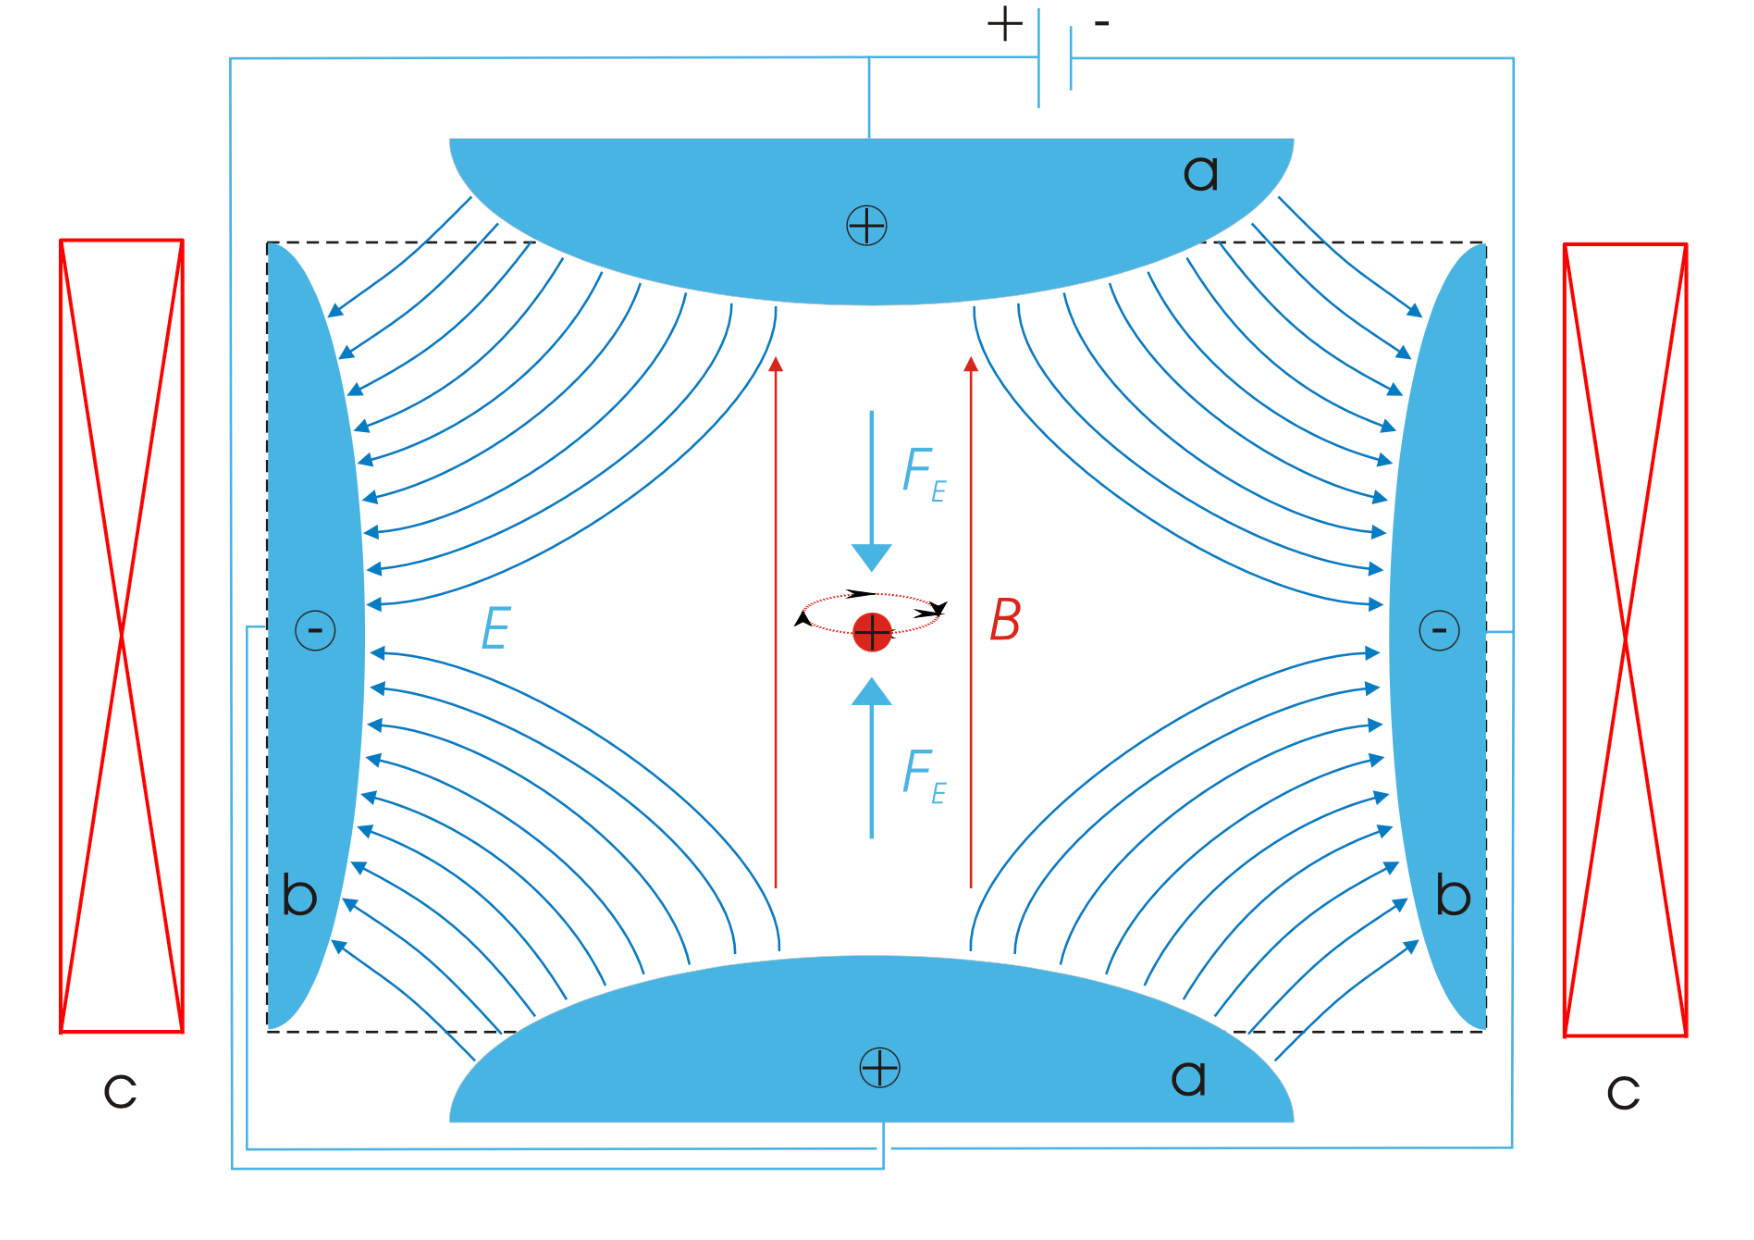
\includegraphics[width=.5\textwidth]{../figures/Penning_trap.pdf}
    \caption{This figure shows the idea of a Penning trap with a red positively charged particle in the center. 
    Here blue lines represent the electric field generated by a quadrupole consisting of end caps (a) and a ring electrode (b). 
    The red lines represent the magnetic field created by a surrounding cylinder magnet (c). 
    Illustration by Arian Kriesch taken from Wikimedia Commons.}
    \label{fig:Penning_trap}
\end{figure}

% ===========================================
\section{Methods}\label{sec:methods}
The physical laws used to implement the Penning trap simulation will be from electrodynamics and classical mechanics, we will not take quantum aspects into account.
The following equations will be used:

\begin{equation}\label{eq:el_field}
    \textbf{E} = - \nabla V
\end{equation}
$\textbf{E}$ is the electric field and $V$ the electric potential.

\begin{equation}\label{eq:el_at_r}
    \textbf{E(r)} = k_e \sum_{j=1}^{n} q_j \frac{\textbf{r} - \textbf{r}_j}{|\textbf{r} - \textbf{r}_j|^3}
\end{equation}
$\textbf{E(r)}$ is the electric field at a point \textbf{r}. This is set up by point charges ${q_1,...,q_n}$ at points ${\textbf{r}_1,...,\textbf{r}_n}$. This comes from \textbf{Coulomb's law}, stating the magnitude of force between to point charges. $k_e \approx 8.988 \cdot 10^9 N m^2 C^{-2}$ is the Coulomb constant.  

\begin{equation}\label{eq:lorentz}
    \textbf{F} = q\textbf{E} + q \textbf{v} \cross \textbf{B}
\end{equation}
This is the $\textbf{Lonretz force}$, the force $\textbf{F}$ on a particle 
with charge $q$, an electric field \textbf{E}, magnetic field \textbf{B} and velocity of the particle \textbf{v}.

\begin{equation}\label{eq:N2L}
    m \ddot{\textbf{r}} = \sum_i \textbf{F}_i
\end{equation}
Eq. \ref*{eq:N2L} is Newton's second law. Here $m$ is the mass of the particle and $\ddot{\textbf{r}} \equiv \frac{d^2 \textbf{r}}{dt^2}$ (the acceleration). 
Famously expressing that the sum of forces equals mass times acceleration.

\begin{equation}\label{eq:el_potential}
    V(x,y,z) = \frac{V_0}{2d^2} (2z^2 - x^2 - y^2)
\end{equation}
For this experiment we will be considering an ideal Penning trap for which the electric field $\textbf{E}$ is given by the electric potential $V$. 
Here $V_0$ is the potential applied to the electrodes. $d = \sqrt{z_0^2 + r_0^2 / 2}$ is the $\textit{charachteristic dimension}$ representing the length scale 
for the region between electrodes. Here $z_0$ is distance from the center to the end caps (a) and $r_0$ is the distance from the center 
to the surrounding ring (b).

\begin{equation}\label{eq:mag_field}
    \textbf{B} = B_0 \hat{e}_z = (0,0,B_0)
\end{equation}
$\textbf{B}$ is the homogenous magnetic field and is dictated by the field strength $B_0$. With $B_0 > 0$. 

Now starting from Newton's second law and using the equations above we can express the time evolution of the particles motion.
The sum of forces will be the Lonretz force, putting eq. \ref*{eq:lorentz} into eq. \ref*{eq:N2L} leads to:
\begin{equation}\label{eq:N2L_lorentz}
    m \ddot{\textbf{r}} = q\textbf{E} + q \textbf{v} \cross \textbf{B}
\end{equation}
Here $\ddot{\textbf{r}} = (\ddot{x},\ddot{y},\ddot{z})$ and $\textbf{v} = (\dot{x},\dot{y},\dot{z})$. Putting eq. \ref*{eq:el_potential} into eq. \ref*{eq:el_field} gives us:
\begin{equation}\label{eq:el_calculated}
    \textbf{E} = \left( x \frac{v_0}{d^2}, y \frac{v_0}{d^2}, -2z \frac{v_0}{d^2} \right)
\end{equation}
Now looking at $q \textbf{v} \cross \textbf{B}$ we have:
\begin{equation}\label{eq:cross_calculated}
    (q \dot{x},q \dot{y},q \dot{z}) \cross (0, 0, B_0) = (B_0 q \dot{y}, -B_0 q \dot{x}, 0)
\end{equation}
Finally substituting for $\textbf{E}$ and $q \textbf{v} \cross \textbf{B}$ in eq. \ref*{eq:N2L_lorentz} results in:
\begin{equation*}
    m \begin{pmatrix}
        \ddot{x} \\ \\ \ddot{y} \\ \\ \ddot{z}
    \end{pmatrix}
    = \begin{pmatrix}
        q x \frac{v_0}{d^2} \\ \\ q y \frac{v_0}{d^2} \\ \\ -2 q z \frac{v_0}{d^2}
    \end{pmatrix}
    + \begin{pmatrix}
        B_0 q \dot{y} \\ \\ -B_0 q \dot{x} \\ \\ 0
    \end{pmatrix}
\end{equation*}
Rewriting this as a set of equations leaves us with:
\begin{align}
    \ddot{x} - w_0 \dot{y} - \frac{1}{2}& w_z^2 x = 0 \label{eq:a_x}\\
    \ddot{y} + w_0 \dot{x} - \frac{1}{2}& w_z^2 y = 0 \label{eq:a_y}\\
    \ddot{z} + w_z^2& z = 0 \label{eq:a_z}
\end{align}
Where $w_0 = \frac{qB_0}{m}$ and $w_z^2 = \frac{2qV_0}{md^2}$. Taking a closer look at eq. \ref*{eq:a_z} we see that the general solution is:
\begin{equation}
    z = A \cos(w_z^2 t) + B \sin(w_z^2 t)
\end{equation}
eq. \ref*{eq:a_x} and \ref*{eq:a_y} are coupled, thus introducing a challenge. This can be resolved by introducing a complex function $f(t) = x(t) + iy(t)$ and rewriting them as a single differential equation. By introducing the complex function we have:
\begin{align}
    f(t) = x(t) + iy(t) \\
    \dot{f}(t) = \dot{x}(t) + i\dot{y}(t) \\
    \ddot{f}(t) = \ddot{x}(t) + i\ddot{y}(t)
\end{align}
Now multiplying eq. \ref*{eq:a_y} by $i$ gives:
\begin{equation}
    i\ddot{y} + iw_0 \dot{x} - i\frac{1}{2} w_z^2 y = 0 \label{eq:a_iy}
\end{equation}
eq. \ref*{eq:a_x} and \ref*{eq:a_iy} can then be summed:
\begin{equation}
    \ddot{x}+ i\ddot{y} - w_0 \dot{y} + iw_0 \dot{x} - \frac{1}{2} w_z^2 x - i\frac{1}{2} w_z^2 y= 0
\end{equation}
Finally, substituting for $f(t)$, $\dot{f}(t)$ and $\ddot{f}(t)$ shows that eq. \ref*{eq:a_x} and \ref*{eq:a_y} can be rewritten as a single differential equation for $f$:
\begin{equation}
    \ddot{f} + i w_0 \dot{f} - \frac{1}{2} w_z^2 f = 0 \label{eq:single_diff}
\end{equation}

The general solution to eq. \ref*{eq:single_diff} is:
\begin{equation}
    f(t) = A_+ e^{-i(w_+ t + \phi_+)} + A_- e^{-i(w_- t + \phi_-)} \label{eq:general_sol_f}
\end{equation}
where the amplitudes $A_+$ and $A_-$ are positive, $\phi_+$ and $\phi_-$ are constant phases, and
\begin{equation}
    w_\pm = \frac{w_0 \pm \sqrt{w_0^2 - 2 w_z^2}}{2}
\end{equation}
To obtain a bounded solution for the radial movement ($xy$-plane) of the particle we need to introduce some constraints on $w_0$ and $w_z$. In other words we will introduce some constraints that will ensure that $|f(t)| < \infty$ as $t \rightarrow \infty$.

Studying eq. \ref*{eq:general_sol_f} one notices that $|f(t)| \rightarrow \infty$ only if $w_\pm$ is complex. To avoid this, we introduce the limitation $w_0^2 - 2 w_z^2 \geq 0$, avoiding any negative values inside the square root and consequently limiting the result to real numbers. Rearranging this and remembering that $w_0 = \frac{qB_0}{m}$ and $w_z^2 = \frac{2qV_0}{md^2}$ leaves us with:
\begin{equation}
    \frac{q}{m} \geq \frac{4 V_0}{B_0^2 d^2}
\end{equation}
A constraint, that if satisfied, keeps the particle within the Penning trap.

Now to express the upper and lower bounds of the particles' distance from the origin in the $xy$-plane 
we start with eq. \ref*{eq:general_sol_f}. Through Taylor expansion of $e^{ix}$ we arrive at Euler's formula:
\begin{equation*}
    e^{ix} = \cos(x) + i \sin(x)
\end{equation*} 
Introducing $u =  w_+ t + \phi_+$ and $v = w_- t + \phi_-$, and using 
Euler's formula, eq. \ref*{eq:general_sol_f} can be rewritten as:
\begin{equation*}
    f(t) = A_+\left(\cos(u) - i \sin(u) \right) + A_-\left(\cos(v) - i \sin(v) \right)
\end{equation*}
The physical coordinates can then be found as $x(t) = \Re f(t)$ and  $y(t) = \Im f(t)$. Giving us:
\begin{align*}
    x(t) &= A_+ \cos(u) + A_- \cos(v) \\
    y(t) &= -A_+ \sin(u) - A_- \sin(v)
\end{align*}
Since our $xy$-plane is a circle, the particle's distance from the origin can be expressed as the radius $R = \sqrt{x^2 + y^2}$. 
Substituting for $x$ and $y$ we have:
\begin{align*}
    R = \sqrt{(A_+ \cos(u) + A_- \cos(v))^2} \\ \overline{+ (-A_+ \sin(u) - A_- \sin(v))^2}
\end{align*}
After expanding and rearranging we have:
\begin{align*}
   R = \sqrt{A_+^2(\cos^2(u) + \sin^2(u)) + A_-^2(\cos^2(v) + \sin^2(v))} \\ \overline{ + 2 A_+ A_- (cos(u)\cos(v) + \sin(u)\sin(v))}
\end{align*}
Recognizing that $cos^2(u) + \sin^2(u) = 1$ and $cos(u)\cos(v) + \sin(u)\sin(v) = \cos(u-v)$ this can be simplified to:
\begin{align*}
    R = \sqrt{A_+^2 + A_-^2 + 2 A_+ A_- \cos(u-v)}
\end{align*}
We know that $\cos$ is a function with an upper bound of $1$ and lower bound of $-1$. 
The possible bounds for $R$ are consequently:
\begin{align*}
    R_+ &= \sqrt{A_+^2 +2A_+ A_- + A_-^2} = A_+ + A_- \\
    R_- &= \sqrt{A_+^2 -2A_+ A_- + A_-^2} = |A_+ - A_-|
\end{align*}
% ===========================================
\subsection*{The algorithms}
%
% The algorithm for the midpoint rule is summarized in algorithm~\ref{algo:midpointrule}. The basic idea behind the algorithm is to divide the integration range into to $n$ small subintervals of length $h$, and on each such subinterval approximate the function $f(x)$ by a constant function. The value for this constant function is taken to be the value of $f(x)$ evaluated at the midpoint of the given subinterval --- hence the name of the method.
% %
\begin{figure}[H]
% NOTE: We only need \begin{figure} ... \end{figure} here because of a compatability issue between the 'revtex4-1' document class and the 'algorithm' environment.
    \begin{algorithm}[H]
    \caption{Forward Euler method}
    \label{algo:midpointrule}
        \begin{algorithmic}
            \Procedure{Midpoint rule}{$f, a, b, n$}
            \State $I \leftarrow 0$        \Comment{Initialize the integral variable}
            \State $h \leftarrow (b-a)/n$  \Comment{Compute the interval length}
            \For{$i = 1, 2, \ldots, n$}
            \State $x \leftarrow a + (i-1/2)h$  \Comment{Assign $x$ to the midpoint}  %This means x is assigned the value x + ih/2.
            \State $I \leftarrow I + f(x)$  \Comment{Add contribution to integral} %Assign I to I + f(x)
            \EndFor
            \State $I \leftarrow Ih$  \Comment{Finalize the computation}
            \EndProcedure
        \end{algorithmic}
    \end{algorithm}
\end{figure}

\begin{figure}[H]
    % NOTE: We only need \begin{figure} ... \end{figure} here because of a compatability issue between the 'revtex4-1' document class and the 'algorithm' environment.
        \begin{algorithm}[H]
        \caption{Runge-Kutta fourth order method}
        \label{algo:midpointrule}
            \begin{algorithmic}
                \Procedure{Midpoint rule}{$f, a, b, n$}
                \State $I \leftarrow 0$        \Comment{Initialize the integral variable}
                \State $h \leftarrow (b-a)/n$  \Comment{Compute the interval length}
                \For{$i = 1, 2, \ldots, n$}
                \State $x \leftarrow a + (i-1/2)h$  \Comment{Assign $x$ to the midpoint}  %This means x is assigned the value x + ih/2.
                \State $I \leftarrow I + f(x)$  \Comment{Add contribution to integral} %Assign I to I + f(x)
                \EndFor
                \State $I \leftarrow Ih$  \Comment{Finalize the computation}
                \EndProcedure
            \end{algorithmic}
        \end{algorithm}
    \end{figure}
% \textit{As demonstrated in algorithm~\ref{algo:midpointrule}, it is conventional to present algorithms in a way that is independent of any specific programming language. This ensures that it is the logic behind the algorithm that remains in focus, rather than the syntax of a particular programming language. In algorithm~\ref{algo:midpointrule} we have also demonstrated a common notation: The right-to-left arrow ($\leftarrow$) means that we assign the value of everything on the right to the variable on the left. This is nothing but how the ``='' symbol functions in most programming languages, but the arrow notation makes it clear that we are in fact assigning a value, rather than stating that two things are equal.}


% % ===========================================
\section{Results}\label{sec:results}
% %
% To test the midpoint rule algorithm, we perform the integration of $f(x)$ using different choices for the number of subintervals. The results are listed in table \ref{tab:midpointruletab}.\footnote{A general style recommendation is to avoid having vertical lines in tables. There are of course exceptions, but in most cases vertical lines will make a table less readable.}
% %
% \begin{table}[h!]
%     \centering
%     \caption{Approximate values for the integral of $f(x) = x^3$ on the interval $[0,1]$, as obtained with the midpoint rule with different numbers of integration subintervals.}
%     \begin{tabular}{c@{\hspace{1cm}} c}
%         \hline
%         Number of subintervals & Integral value \\
%         \hline
%         $10^1$  &  0.3086 \\
%         $10^2$  &  0.2550 \\
%         $10^3$  &  0.2505 \\
%         $10^4$  &  0.2500 \\
%         % $10$  &  0.3086 \\
%         % $100$  &  0.2550 \\
%         % $1 000$  &  0.2505 \\
%         % $10 000$  &  0.2500 \\
%         \hline
%     \end{tabular}\label{tab:midpointruletab}
% \end{table}

% In figure \ref{fig:rel_err} we show the relative error as a function of the number of subintervals $n$.
% \begin{figure}[h!]
%     \centering %Centers the figure
%     %\includegraphics[scale=0.55]{} %Imports the figure.
%     \caption{The relative error versus the number of integration subintervals ($n$) when using the midpoint rule to estimate the integral $\int_0^1 x^3\dd x$. \textit{Given that this plot is based only on a handful of data points, it should also show the data points using some form of point markers, like the dots here. When presented only with a continuous line, it is not necessarily clear for the reader if the result is based on a large or small number of data points.}}
%     \label{fig:rel_err}
% \end{figure}

% \textit{Note especially how we reference both the table and the figure with a short explanation of their content. Always do this! In the figure/table captions we can also add additional information, such as information about how the figure/table was produced. You can also do this in the main text if you like. When writing the figure/table captions, keep in mind the general rule of thumb that an expert on the topic should be able to understand the gist of your report simply by reading the abstract and look at the figures/tables and read their corresponding captions.}


% ===========================================
\section{Discussion}\label{sec:discussion}
%
\textit{Note that you are free to merge the presentation and discussion of the results into a single section of your report. This can in many cases lead to a more fluid presentation. If you do this, we recommend you use ``Results and discussion'' or similar for the section title.}

From table \ref{tab:midpointruletab}, we note that our implementation reproduces the analytical results to four digits precision when the integration range is divided into $n = 10^4$ subintervals. This indicates that that our implementation of the algorithm is correct.

From figure \ref{fig:rel_err}, we see that $\log_{10}(\epsilon)$ decreases linearly with $\log_{2}(n)$. From this, it should be possible to extract the convergence rate of our implementation of the midpoint rule. From a theoretical point of view we know that the midpoint rule should have a convergence rate of $\mathcal{O}(h^2)$. To properly verify our implementation, we should have estimated the convergence rate from our results and compared it to this theoretical rate. Without doing so, we cannot know that the our implementation of the algorithm is correct, even though we have seen that the numerical approximation converges to the correct answer in \ref{tab:midpointruletab}.

\textit{Although this is a somewhat silly example, please note the following: We are to-the-point in our discussion of the results, and we only make strong claims about what we are actually certain about. In the discussion it is important to try to be as concise as possible --- long paragraphs that only make very general points are typically of limited interest. Note that we also highlight aspects of our analysis that could have been improved and that might form a topic for future work.}


% ===========================================
\section{Conclusion}\label{sec:conclusion}
\textit{In this section we state three things in a concise manner: what we have done, what we have found, and what should or could be done in the future.}

We have investigated an implementation of the midpoint rule for numerical integration. As a first validation test we have checked that our implementation of the method reproduces the analytical result for the definite integral of $f(x) = x^3$ on $x \in [0,1]$, achieving a four-digit precision when the integration range is divided into $n=10^4$ subintervals. Furthermore, we have presented results for how the relative error of the method varies with the number of subintervals. To use these results to extract a precise estimate for the convergence rate of the method remains a topic for future work. As such, while our implementation of the midpoint rule has passed the initial validation tests, more work is needed to fully assess the validity of the implementation.

\onecolumngrid

%\bibliographystyle{apalike}
\bibliography{ref}


\end{document}
